\documentclass[a4paper,12pt]{article}
\usepackage{amsmath, amssymb}
\usepackage{xcolor}
\usepackage[most]{tcolorbox}
\usepackage{multicol}
\usepackage{geometry}
\usepackage{graphicx}
\usepackage{hyperref}
\graphicspath{ {../Images/} }

\geometry{left=1.5cm, right=1.5cm, top=1.5cm, bottom=1.5cm}

\title{Exercices de Nombres Complexes}
\author{}
\date{}

% Style de boîte pour les exercices
\tcbset{
    colframe=purple!70,
    colback=white,
    coltitle=black,
    fonttitle=\bfseries,
    sharp corners,
    boxrule=0.5mm,
    colbacktitle=purple!20!white,
    center title,
    boxsep=4pt,
}

% Style de boîte pour les solutions
\newtcolorbox{solutionbox}[1][]{
    colframe=green!70,
    colback=white,
    coltitle=black,
    fonttitle=\bfseries,
    sharp corners,
    boxrule=0.5mm,
    colbacktitle=green!20!white,
    title=Solution,
    boxsep=4pt,
    breakable,
    #1
}

\begin{document}

% Exercice 17
\begin{tcolorbox}[title={Exercice 17 - {[}Représenter, Calculer, Chercher{]}}]
Dans un repère orthonormé, peut-on trouver un triangle équilatéral dont les trois sommets sont à coordonnées entières ?
\end{tcolorbox}

\begin{solutionbox}
\textbf{Solution :}

Supposons qu'il existe un triangle équilatéral \( ABC \) dont les sommets ont des coordonnées entières.

Représentons les sommets par des nombres complexes :

Soit \( z_A = x_A + i y_A \), \( z_B = x_B + i y_B \), \( z_C = x_C + i y_C \), avec \( x_A, y_A, x_B, y_B, x_C, y_C \in \mathbb{Z} \).

Dans un triangle équilatéral, les côtés sont de même longueur, et les vecteurs côtés sont obtenus par rotation de \( 120^\circ \) (ou \( \dfrac{2\pi}{3} \) radians).

Considérons le vecteur \( \overrightarrow{AB} = z_B - z_A \).

Alors, le vecteur \( \overrightarrow{AC} \) est obtenu en faisant tourner \( \overrightarrow{AB} \) de \( 60^\circ \) (ou \( \dfrac{\pi}{3} \) radians) :

\[
\overrightarrow{AC} = e^{i\frac{\pi}{3}} (\overrightarrow{AB})
\]

Donc :

\[
z_C - z_A = e^{i\frac{\pi}{3}} (z_B - z_A)
\]

Ce qui donne :

\[
z_C = z_A + e^{i\frac{\pi}{3}} (z_B - z_A)
\]

Développons :

\[
z_C = z_A + \left( \cos\left( \dfrac{\pi}{3} \right) + i \sin\left( \dfrac{\pi}{3} \right) \right) (z_B - z_A)
\]

Or, \( \cos\left( \dfrac{\pi}{3} \right) = \dfrac{1}{2} \) et \( \sin\left( \dfrac{\pi}{3} \right) = \dfrac{\sqrt{3}}{2} \).

Donc :

\[
z_C = z_A + \left( \dfrac{1}{2} + i \dfrac{\sqrt{3}}{2} \right) (z_B - z_A)
\]

Comme \( z_A \) et \( z_B \) ont des coordonnées entières, \( z_B - z_A \) a des coordonnées entières.

Cependant, en multipliant \( z_B - z_A \) par \( \dfrac{1}{2} + i \dfrac{\sqrt{3}}{2} \), nous obtenons un nombre complexe dont les parties réelles et imaginaires sont des combinaisons linéaires des coordonnées entières multipliées par \( \dfrac{1}{2} \) et \( \dfrac{\sqrt{3}}{2} \), c'est-à-dire des nombres qui ne sont pas entiers (car \( \dfrac{\sqrt{3}}{2} \) est irrationnel).

Par conséquent, \( z_C \) aura des coordonnées non entières.

\textbf{Conclusion :} Il est impossible de construire un triangle équilatéral dont les trois sommets ont des coordonnées entières dans un repère orthonormé.

\end{solutionbox}


% Exercice 19
\begin{tcolorbox}[title=Exercice 19]
Le plan complexe est muni d'un repère orthonormé \( (O ; \vec{u}, \vec{v}) \) et on considère les points \( A \), \( B \) et \( C \) d'affixes respectives :  
\( z_A = \sqrt{2}e^{-\frac{3i\pi}{4}} \), \( z_B = 3 + 3i \) et \( z_C = 7 - i \).

\begin{enumerate}
    \item Déterminer la forme algébrique de \( z_A \) et une forme exponentielle de \( z_B \).
    \item Quelle est la nature du triangle \( ABC \) ?
    \item Démontrer qu'il existe un point \( D \) tel que le quadrilatère \( ABCD \) soit un carré. Déterminer l'affixe du point \( D \).
    \item Déterminer l'affixe du centre du carré \( ABCD \).
    \item On considère l'ensemble des points \( M \) du plan d'affixe \( z \) tels que \( |z - (3 - i)| = 4 \). Démontrer que cet ensemble est le cercle circonscrit au triangle \( ABC \).
\end{enumerate}
\end{tcolorbox}

\begin{solutionbox}
\begin{enumerate}
    \item \textbf{Forme algébrique de \( z_A \) et forme exponentielle de \( z_B \) :}

    \textbf{Pour \( z_A \) :}

    \[
    z_A = \sqrt{2} e^{-i\frac{3\pi}{4}} = \sqrt{2} \left[ \cos\left( -\dfrac{3\pi}{4} \right) + i \sin\left( -\dfrac{3\pi}{4} \right) \right]
    \]

    Calculons :

    \[
    \cos\left( -\dfrac{3\pi}{4} \right) = -\dfrac{\sqrt{2}}{2}, \quad \sin\left( -\dfrac{3\pi}{4} \right) = -\dfrac{\sqrt{2}}{2}
    \]

    Donc :

    \[
    z_A = \sqrt{2} \left( -\dfrac{\sqrt{2}}{2} - i \dfrac{\sqrt{2}}{2} \right) = (-1 - i)
    \]

    \textbf{Pour \( z_B \) :}

    Calculons le module et l'argument de \( z_B = 3 + 3i \).

    Module :

    \[
    |z_B| = \sqrt{3^2 + 3^2} = 3\sqrt{2}
    \]

    Argument :

    \[
    \theta = \dfrac{\pi}{4}
    \]

    Donc :

    \[
    z_B = 3\sqrt{2} e^{i\frac{\pi}{4}}
    \]

    \item \textbf{Nature du triangle \( ABC \) :}

    Calculons les vecteurs :

    \[
    \overrightarrow{AB} = z_B - z_A = (3 + 3i) - (-1 - i) = 4 + 4i
    \]

    \[
    \overrightarrow{AC} = z_C - z_A = (7 - i) - (-1 - i) = 8 + 0i = 8
    \]

    Calculons les longueurs :

    \[
    AB = \sqrt{4^2 + 4^2} = \sqrt{16 + 16} = \sqrt{32}
    \]

    \[
    AC = |8| = 8
    \]

    \[
    BC = |z_C - z_B| = |(7 - i) - (3 + 3i)| = |4 - 4i| = \sqrt{4^2 + (-4)^2} = \sqrt{32}
    \]

    Donc \( AB = BC = \sqrt{32} \).

    Calculons \( AC^2 = 64 \) et \( AB^2 = BC^2 = 32 \).

    Vérifions le théorème de Pythagore :

    \[
    AB^2 + BC^2 = 32 + 32 = 64 = AC^2
    \]

    Donc, le triangle \( ABC \) est rectangle en \( B \).

    \textbf{Conclusion :} Le triangle \( ABC \) est isocèle rectangle en \( B \).

    \item \textbf{Existence du point \( D \) tel que \( ABCD \) soit un carré :}

    Puisque \( ABC \) est un triangle rectangle isocèle, en ajoutant le point \( D \) tel que \( ABCD \) soit un carré, nous pouvons déterminer \( z_D \).

    Le vecteur \( \overrightarrow{CD} \) est égal au vecteur \( \overrightarrow{AB} \).

    Donc :

    \[
    z_D = z_C + (z_A - z_B) = z_C + (-\overrightarrow{AB})
    \]

    Calculons :

    \[
    z_D = z_C - (z_B - z_A) = (7 - i) - [(3 + 3i) - (-1 - i)] = (7 - i) - (4 + 4i) = (3 - 5i)
    \]

    \item \textbf{Affixe du centre du carré \( ABCD \) :}

    Le centre \( O \) du carré est le milieu des diagonales \( AC \) ou \( BD \).

    Calculons :

    \[
    z_O = \dfrac{z_A + z_C}{2} = \dfrac{(-1 - i) + (7 - i)}{2} = \dfrac{6 - 2i}{2} = 3 - i
    \]

    \item \textbf{Montrer que \( |z - (3 - i)| = 4 \) est le cercle circonscrit au triangle \( ABC \) :}

    Calculons les distances de \( A \), \( B \) et \( C \) au point \( O = 3 - i \):

    Pour \( A \) :

    \[
    |z_A - z_O| = |(-1 - i) - (3 - i)| = |-4| = 4
    \]

    Pour \( B \) :

    \[
    |z_B - z_O| = |(3 + 3i) - (3 - i)| = |4i| = 4
    \]

    Pour \( C \) :

    \[
    |z_C - z_O| = |(7 - i) - (3 - i)| = |4| = 4
    \]

    Ainsi, les trois sommets \( A \), \( B \), \( C \) sont situés à une distance de 4 du point \( O = 3 - i \).

    \textbf{Conclusion :} Le cercle de centre \( 3 - i \) et de rayon 4 est le cercle circonscrit au triangle \( ABC \).
\end{enumerate}
\end{solutionbox}


% Exercice 21
\begin{tcolorbox}[title={Exercice 21}]
Soit \( z = x + iy \) un nombre complexe, où \( x \) et \( y \) sont des nombres réels.  
À tout nombre complexe \( z \), on associe le nombre noté \( e^z \) défini par \( e^z = e^x (\cos y + i \sin y) \).

\begin{enumerate}
    \item Vérifier que pour tous nombres complexes \( z_1 \) et \( z_2 \), on a : \( e^{z_1} \times e^{z_2} = e^{z_1 + z_2} \).
    \item Écrire la forme algébrique de \( e^{2 + 3i} \).
    \item Déterminer une solution de l'équation \( e^z = 1 + i\sqrt{3} \). En existe-t-il d'autres ?
\end{enumerate}
\end{tcolorbox}

\begin{solutionbox}
\begin{enumerate}
    \item \textbf{Vérification de la propriété exponentielle pour les nombres complexes :}

    Soient \( z_1 = x_1 + i y_1 \) et \( z_2 = x_2 + i y_2 \), avec \( x_1, y_1, x_2, y_2 \in \mathbb{R} \).

    Calculons \( e^{z_1} \times e^{z_2} \) :

    \[
    e^{z_1} \times e^{z_2} = e^{x_1} (\cos y_1 + i \sin y_1) \times e^{x_2} (\cos y_2 + i \sin y_2) = e^{x_1 + x_2} [ (\cos y_1 + i \sin y_1)(\cos y_2 + i \sin y_2) ]
    \]

    Calculons le produit des deux expressions trigonométriques :

    \[
    (\cos y_1 + i \sin y_1)(\cos y_2 + i \sin y_2) = \cos y_1 \cos y_2 - \sin y_1 \sin y_2 + i (\cos y_1 \sin y_2 + \sin y_1 \cos y_2)
    \]

    Rappelons les formules d'addition :

    \[
    \cos(y_1 + y_2) = \cos y_1 \cos y_2 - \sin y_1 \sin y_2
    \]
    \[
    \sin(y_1 + y_2) = \sin y_1 \cos y_2 + \cos y_1 \sin y_2
    \]

    Donc :

    \[
    (\cos y_1 + i \sin y_1)(\cos y_2 + i \sin y_2) = \cos(y_1 + y_2) + i \sin(y_1 + y_2)
    \]

    Ainsi :

    \[
    e^{z_1} \times e^{z_2} = e^{x_1 + x_2} [ \cos(y_1 + y_2) + i \sin(y_1 + y_2) ] = e^{(x_1 + x_2) + i (y_1 + y_2)} = e^{z_1 + z_2}
    \]

    \textbf{Conclusion :} La propriété exponentielle est vérifiée pour les nombres complexes.

    \item \textbf{Forme algébrique de \( e^{2 + 3i} \) :}

    On a \( z = 2 + 3i \), donc \( x = 2 \) et \( y = 3 \).

    Alors :

    \[
    e^z = e^{2} (\cos 3 + i \sin 3)
    \]

    Calculons \( \cos 3 \) et \( \sin 3 \) (les valeurs numériques) :

    \[
    \cos 3 \approx \cos 3 \text{ radians} \approx -0.9900
    \]
    \[
    \sin 3 \approx \sin 3 \text{ radians} \approx 0.1411
    \]

    Donc :

    \[
    e^{2 + 3i} \approx e^{2} ( -0.9900 + i \times 0.1411 ) \approx e^{2} ( -0.9900 + 0.1411 i )
    \]

    Calculons \( e^{2} \approx 7.3891 \)

    Donc :

    \[
    e^{2 + 3i} \approx 7.3891 ( -0.9900 + 0.1411 i ) \approx -7.306 + 1.043 i
    \]

    \textbf{Conclusion :} \( e^{2 + 3i} \approx -7.306 + 1.043 i \)

    \item \textbf{Résolution de l'équation \( e^{z} = 1 + i\sqrt{3} \) :}

    Soit \( z = x + i y \), avec \( x, y \in \mathbb{R} \).

    On a :

    \[
    e^{x} (\cos y + i \sin y) = 1 + i\sqrt{3}
    \]

    Écrivons le second membre en forme exponentielle :

    Calculons le module et l'argument de \( 1 + i\sqrt{3} \).

    Module :

    \[
    r = |1 + i\sqrt{3}| = \sqrt{1^2 + (\sqrt{3})^2} = \sqrt{1 + 3} = \sqrt{4} = 2
    \]

    Argument :

    \[
    \theta = \arctan\left( \dfrac{\sqrt{3}}{1} \right) = \dfrac{\pi}{3}
    \]

    Donc :

    \[
    1 + i\sqrt{3} = 2 \left( \cos \dfrac{\pi}{3} + i \sin \dfrac{\pi}{3} \right)
    \]

    Donc, l'équation devient :

    \[
    e^{x} (\cos y + i \sin y) = 2 \left( \cos \dfrac{\pi}{3} + i \sin \dfrac{\pi}{3} \right)
    \]

    En identifiant les modules et les arguments, on a :

    \[
    e^{x} = 2
    \]
    \[
    y = \dfrac{\pi}{3} + 2k\pi, \quad k \in \mathbb{Z}
    \]

    Donc :

    \[
    x = \ln 2
    \]
    \[
    y = \dfrac{\pi}{3} + 2k\pi, \quad k \in \mathbb{Z}
    \]

    \textbf{Conclusion :} Les solutions de l'équation sont \( z = \ln 2 + i \left( \dfrac{\pi}{3} + 2k\pi \right) \), avec \( k \in \mathbb{Z} \).

    \textbf{Il existe une infinité de solutions} car l'argument peut être augmenté de \( 2\pi \) sans changer la valeur de \( e^{z} \).

\end{enumerate}
\end{solutionbox}

% Exercice 22
\begin{tcolorbox}[title={Exercice 22}]
\begin{center}
    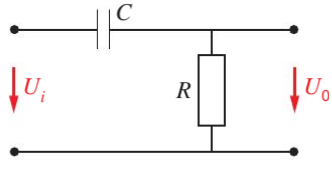
\includegraphics[width=0.5\textwidth]{schema_exo65.png}
\end{center}
En électricité, en régime sinusoïdal utilisant un courant alternatif de pulsation \( \omega \), on utilise les nombres complexes pour représenter les tensions et intensités sinusoïdales.  
On sait, grâce aux lois de l'électricité, que la tension complexe \( U_0 \) aux bornes de la résistance \( R \) est reliée à l'intensité complexe \( I \) par la relation \( U_0 = R I \) et que
\[
U_i = \dfrac{1}{i C \omega} I + U_0,
\]
où \( C \) est la capacité du condensateur.

On cherche le gain du circuit : \( G = \dfrac{U_0}{U_i} \).

\begin{enumerate}
    \item Démontrer que
       \[
       G = \dfrac{i R C \omega}{1 + i R C \omega}.
       \]
    \item Quand \( R = 1000 \) ohms, \( C = 64 \times 10^{-6} \) farads et \( \omega = 60000 \) Hz, démontrer que le module de \( G \) est proche de 1.
    \item Rechercher le sens de « circuit passe-haut ».
\end{enumerate}

\end{tcolorbox}

\begin{solutionbox}
\begin{enumerate}
    \item \textbf{Expression du gain \( G \) :}

    Commençons par exprimer \( U_i \) en fonction de \( I \) :

    \[
    U_i = \dfrac{1}{i C \omega} I + U_0 = \dfrac{1}{i C \omega} I + R I = \left( \dfrac{1}{i C \omega} + R \right) I
    \]

    Mettons sur un dénominateur commun :

    \[
    \dfrac{1}{i C \omega} + R = \dfrac{1 + i R C \omega}{i C \omega}
    \]

    Ainsi :

    \[
    U_i = \left( \dfrac{1 + i R C \omega}{i C \omega} \right) I
    \]

    Or, \( U_0 = R I \).

    Donc, le gain est :

    \[
    G = \dfrac{U_0}{U_i} = \dfrac{R I}{\left( \dfrac{1 + i R C \omega}{i C \omega} \right) I} = \dfrac{R}{\dfrac{1 + i R C \omega}{i C \omega}} = R \times \dfrac{i C \omega}{1 + i R C \omega}
    \]

    Simplifions :

    \[
    G = \dfrac{i R C \omega}{1 + i R C \omega}
    \]

    \textbf{Conclusion :} On a démontré que \( G = \dfrac{i R C \omega}{1 + i R C \omega} \).

    \item \textbf{Calcul du module de \( G \) :}

    Données :

    \[
    R = 1000 \, \Omega, \quad C = 64 \times 10^{-6} \, \text{F}, \quad \omega = 60000 \, \text{rad/s}
    \]

    Calculons \( R C \omega \) :

    \[
    R C \omega = 1000 \times 64 \times 10^{-6} \times 60000 = 1000 \times (64 \times 10^{-6} \times 60000)
    \]

    Calculons \( 64 \times 10^{-6} \times 60000 \) :

    \[
    64 \times 10^{-6} \times 60000 = 64 \times 6 \times 10^{-6} \times 10^{4} = 64 \times 6 \times 10^{-2} = 384 \times 10^{-2} = 3.84
    \]

    Donc :

    \[
    R C \omega = 1000 \times 3.84 = 3840
    \]

    Ainsi, \( R C \omega = 3840 \).

    Alors :

    \[
    G = \dfrac{i \times 3840}{1 + i \times 3840} = \dfrac{i \times 3840}{1 + i \times 3840}
    \]

    Calculons le module de \( G \) :

    Le module de \( G \) est :

    \[
    |G| = \dfrac{|i \times 3840|}{\sqrt{1^2 + (3840)^2}} = \dfrac{3840}{\sqrt{1 + 3840^2}}
    \]

    Calculons \( \sqrt{1 + 3840^2} \) :

    \[
    \sqrt{1 + 3840^2} = \sqrt{1 + 14,745,600} = \sqrt{14,745,601} \approx 3840.00013
    \]

    Donc :

    \[
    |G| = \dfrac{3840}{3840.00013} \approx 0.99999997 \approx 1
    \]

    \textbf{Conclusion :} Le module de \( G \) est très proche de 1.

    \item \textbf{Sens de « circuit passe-haut » :}

    Un circuit passe-haut est un filtre qui laisse passer les hautes fréquences et atténue les basses fréquences.

    Dans notre cas, lorsque \( \omega \) est très grand, \( R C \omega \) est grand, et \( |G| \) tend vers 1.

    Lorsque \( \omega \) est petit, \( R C \omega \) est petit, et le module de \( G \) est faible.

    Ainsi, le circuit transmet bien les hautes fréquences (gain proche de 1) et atténue les basses fréquences (gain proche de 0).

    \textbf{Conclusion :} Le circuit est un filtre passe-haut, laissant passer les hautes fréquences.

\end{enumerate}
\end{solutionbox}


\end{document}

\end{document}